\documentclass[12pt,oneside,final]{siuethesis}
\usepackage{microtype} % (optional) for more beautiful typesetting
\usepackage{graphicx} 
\usepackage{hyperref} %makes links clickable
\hypersetup{colorlinks,citecolor=black,filecolor=black,linkcolor=blue,urlcolor=black} %good for electronic copy
\hypersetup{colorlinks,citecolor=black,filecolor=black,linkcolor=black,urlcolor=black}%required for paper graduate school copy
%\usepackage[alphabetic]{amsrefs} %required if using amsrefs, comment out if using bibtex
\usepackage{fixltx2e}
\usepackage{amsmath}
\usepackage{epsf}
%\usepackage{float}
\usepackage{caption}
\usepackage{subfig}
%\usepackage{subcaption}
\usepackage{listings}
\usepackage{rotating}
\usepackage{tabularx}
\usepackage{multirow}

%% controls numbering of theorems
%% this can be configured to your advisor's taste
\newtheorem{theorem}{Theorem}[chapter] %theorem number resets each chapter
\newtheorem{conclusion}[theorem]{Conclusion}
\newtheorem{condition}[theorem]{Condition}
%% conjectures, corollary, defn, etc. numbered sequentially from beginning of chapters
\newtheorem{conjecture}[theorem]{Conjecture} 
\newtheorem{corollary}[theorem]{Corollary}
\newtheorem{example}[theorem]{Example} 
\newtheorem{lemma}[theorem]{Lemma}
\newtheorem{proposition}[theorem]{Proposition}
\newtheorem{solution}[theorem]{Solution}
\theoremstyle{definition}
\newtheorem{definition}[theorem]{Definition}


\author{Bryan Orabutt}
\title{Design of a Multichannel Constant Fraction Discriminator IC for Use in Nuclear Physics Applications}

%%\advisor{John Q.\ Faculty} %% or 
\advisor{Dr.}{George L. Engel}
\secondreader{Dr.}{Bradley Noble} %% or \secondreader{Dr.}{Karl Gauss}
\thirdreader{Dr.}{Timothy York}
%\fourthreader{Karl Gauss, Sr.}
%\fifthreader{Karl Gauss, Sr.}
%\secondadvisor{Karl Gauss} %if you haves two advisors (rare) then use this line also and pass the option `twoadvisors' to the class
%\abstracttext{Chairperson: The Honorable Jill Smith} %optional -- you can use this to override the text on the abstract page; the grad school default is built-in
\submitdate{April, 2018} %date the month/year submitted to grad school, use a comma between
\copyrightyear{2018} %optional, but required if copyrighted

%% all of these are optional; defaults are shown
\major{Electrical Engineering} 
\degree{Master of Science} %can be used to specify M.A., etc.
\highestdegree{Bachelor of Science} %used if the author already has another graduate degree
\department{Electrical and Computer Engineering} 
%\departmentname{Department}
%\refname{REFERENCES} 

%\captionsetup{width=0.7\textwidth}

\begin{document}
\maketitle 

\frontmatter %signals single spacing/roman numeral pagination

\copyrightpage %optional

%%% abstracts are optional
\begin{abstract}
\par This thesis presents the design and simulation of a multichannel integrated circuit (IC) that will be used in nuclear physics experiments. The chip is being designed as a companion chip for another IC used in particle identification called PSD8C. The IC described in this thesis is used create precise timing pulses for starting time-to-voltage converters (TVCs) on the PSD8C. These timing pulses are created using a technique called constant fraction discrimination. Each of the sixteen channels in the IC contains a Nowlin circuit, leading edge discriminator, zero cross discriminator, and a one shot circuit to generate the output. \par The IC will support input pulse amplitudes between 20 mV and 2V both positive and negative, and input rise times between 3 nsec and 100 nsec. The IC will feature a programmable output pulse width between 50 nsec and 500 nsec. Most importantly the output pulse firing time variation will be independent of the input amplitude and rise time, having a time walk of only 1 nsec or less. The IC has been named CFD16C and the design presented is using the AMI 0.5 micron NWELL process.

\end{abstract}

\begin{acknowledgements}

\par I would first like to thank Dr. George Engel for being a continuous source of guidance through all my time working on this project. I would also like to thank Dr. Bradley Noble for encouraging me to investigate challenging problems and for being a source of guidance both in the classroom and out. I would also thank Dr. Timothy York for introducing me to IC design, without him I likely would never have gone to graduate school. Additionally, Dr. Gary Mayer of the Computer Science department has helped me expand knowledge beyond the skills learned in the classroom, and I am forever thankful.
\par I would like to thank the other graduate students I've been privileged to work with on this project as well. Pohan Wang, Prarthana Jani, Sneha Edula, and Anil Korkmaz and I all worked together to make CFD16C possible and they have helped make this project a pleasure to work on.
\par I would like to thank my friends Jack White, Jared Charter, and Cameron Costanzo, Nelly Sanchez, and Shana Mankouski for their support during all of my endeavours in graduate school. Finally I am forever grateful to my family for being a constant source of encouragement. My mother Marsha Orabutt, brother Sean Orabutt, and Vicki Kern who has been like a second mother to me, have all been there for me and I know I could not have come this far without them.

\end{acknowledgements}

\tableofcontents

\cleardoublepage %cause correct numbering of list of figures

\listoffigures %print list of figures page

\cleardoublepage

\listoftables

\mainmatter %signals single spacing/arabic numeral paginations


\chapter{INTRODUCTION}  %% chapter titles must be typed in all caps to conform with regulations
\section{Background}
\par This thesis presents the initial design of a multichannel integrated circuit (IC) for use in nuclear physics applications. The IC as of this writing has not been finished and development will continue in a newer design process. The IC will be capable of using constant fraction discrimination (CFD) to create output timing pulses that are independent of input voltage and rise time. The work on this IC has been made possible due to a grant from the National Science Foundation (NSF Grant\#1625499).
\par Collaboration with nuclear physics researchers at Washington University in St. Louis has allowed the design of CFD16C to meet the needs for any experiments involving the PSD8C. The CFD16C is being designed to have better jitter and time walk performance than current existing CFD circuits using VME interface as well as offer functionality tailored to nuclear physics experiments. Combined with its companion ICs the CFD16C will allow for more precise experiments than was previously available.

\section{Need for an Integrated Circuit}
\par There is a need for an IC containing multiple configurable CFD circuits. Other timing ICs and VME CFD circuits do not offer any custom tailored solutions to nuclear physics applications and can limit the scope of an experiment. An IC with the following features is desirable \cite{CFD}:

\begin{itemize}
\item 
Support for up to 16 detectors.
\item
Support amplitudes between 20 mV and 2 V  with between 3 nsec and 100 nsec rise times.
\item
Support for both positive and negative input pulse amplitudes.
\item
Output timing pulse should be independent of input amplitude and rise time.
\item
Configurable leading edge threshold value for each channel.
\item
Programmable output pulse width between 50 nsec and 500 nsec.
\item
Allow for 1 KHz pulse repetition rates.
\end{itemize}

\section{Previous Work}
\par The CFD16C integrated circuit described in this thesis is intended to be used with another microchip (called PSD8C) which employs a technique known as pulse shape discrimination \cite{HALL}. Below is a summarized description of the PSD8C \cite{PROCTOR}. The PSD8C contains eight channels, each containing a time-to-voltage converter (TVC) and three sub channels. The TVC circuits are configurable with two time ranges (0.5 $\mu$sec and 2 $\mu$sec). Each sub channel contains a gated integrator that can be configured with 8 different charging rates, as well as configurable gate generators to set the start and width of the gate relative to the CFD timing pulse (each with 4 time ranges). The PSD8C also has support for 3 triggering modes. The output of a PSD8C channel consists of four sparsified pulse trains (one TVC, three integrators) that are synchronized for digitization by an off chip analog to digital converter (ADC). A system level diagram of the PSD8C is shown in Figure~\ref{fig:PSD} \cite{PSD-NSF}.\newpage

\begin{figure}[ht]
\centering
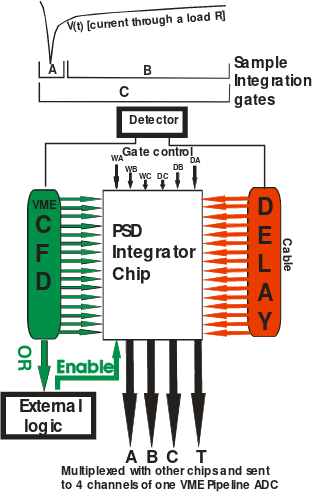
\includegraphics[scale=1,keepaspectratio=true]{images/PSD_block.png} 
\caption{System level overview for the PSD8C}
\label{fig:PSD}
\end{figure}

\par The PSD8C itself is a companion chip for another IC called HINP16C. It is useful to understand HINP16C as well in order to better understand the purpose of CFD16C. HINP16C contains 16 channels for use with silicon strip detectors \cite{HINP}. In each channel there is a charge sensitive amplifier (CSA) with two gain modes. In high gain mode the CSA has a gain of 15 $\frac{mV}{MeV}$ and in low gain it has a gain of 3 $\frac{mV}{MeV}$. The CSA outputs are split and act as inputs to energy and timing branches to produce sparsified pulse train outputs with synchronized addresses for an off chip ADC. 
\par The energy branch consists of a shaping filter that has a return to baseline time of under 20 $\mu$sec. This \emph{slow shaper} circuit is used as input to a continuous-time peak sampling circuit. The timing branch has a pseudo CFD circuit that uses a leading-edge and zero-crossing discriminator. The zero-crossing discriminator makes use of a DC offset cancellation loop to null out any unwanted DC offsets. A DAC is used to correct offsets in the leading-edge discriminator as well as set the CFD threshold level. This CFD output is used to start a TVC circuit with a configurable measurement range (250 nsec and 1 $\mu$sec). This TVC and the peak sampling circuit are reset after a user configurable delay time (referenced to the CFD firing time). A system level diagram of HINP16C is showed in Figure~\ref{fig:HINP} \cite{HINP-THESIS}.

\begin{figure}[ht]
\centering
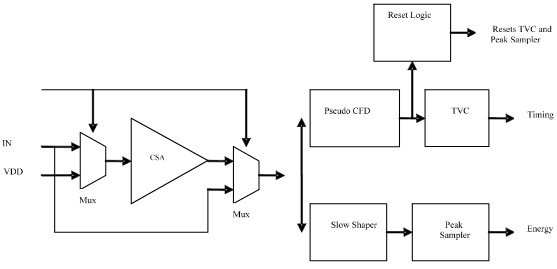
\includegraphics[scale=1,keepaspectratio=true]{images/HINP_block.png} 
\caption{System level overview for the HINP16C}
\label{fig:HINP}
\end{figure}
\par Both PSD8C and HINP16C have been through multiple revisions. PSD8C rev4 was just sent out for fabrication in December of 2017. HINP16C is currently on it's fourth revision with a fifth revision scheduled for the future. In contrast, CFD16C will be an entirely new design.
\section{Scope of Thesis}
\par The object of this thesis work was to begin the design and layout of essential analog elements of the CFD16C (Constant Fraction Discriminator - 16 Channels) integrated circuit. The CFD16C is a companion chip to accompany the PSD8C described in \cite{PROCTOR}. The CFD16C generates the timing pulses needed to start time-to-voltage converters on the PSD8C using a technique called constant fraction discrimination. Information about this technique can be found in \cite{NOWLIN}.
\par The CFD16C is expected to use a 64-pin plastic QFN package. The design will not be continued in the 0.5 micro CMOS process described in this thesis but will be recreated in a newer 0.35 CMOS process. A top level view of the CFD16C described in this thesis is shown in Figure~\ref{fig:CFDtop}.
\par This thesis contains five chapters. Chapter 2 describes the system level overview of the CFD16C. Chapter 3 contains descriptions of the electronic circuits designed for the CFD16C. Chapter 4 contains simulation results showing the circuit elements described in chapter 3 function appropriately. Chapter 5 has a summary, conclusion, and description of future work to be done on the CFD16C.
\vspace{0.25in}
\begin{figure}[ht]
\centering
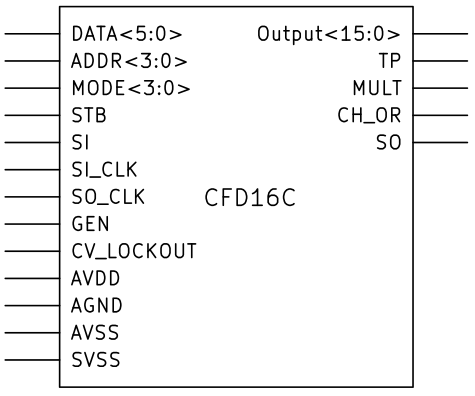
\includegraphics[scale=.8,keepaspectratio=true]{images/CFDtop.png} 
\caption{Top level view of CFD16C showing all inputs and outputs.}
\label{fig:CFDtop}
\end{figure}

\chapter{SYSTEM LEVEL DESIGN}
\section{Overview of Chip}
\par The CFD16C is designed in a 0.5 micron CMOS process. The chip is designed to act as a multichannel constant fraction discriminator with very low jitter and time walk in the output timing pulse. A system level block diagram of a single CFD channel can be seen in Figure~\ref{fig:CFD}.

\begin{figure}[ht]
\centering
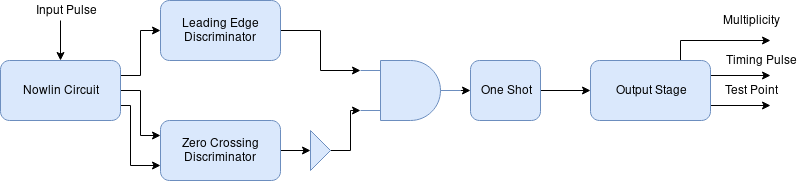
\includegraphics[scale=.55,keepaspectratio=true]{images/CFD.png} 
\caption{System level overview for one channel of the CFD16C}
\label{fig:CFD}
\end{figure}

\par An analog input pulse will arrive at the input stage of of the channel in the form of an exponential voltage pulse with a rise time ~10 times faster than its fall time. This input pulse goes to a Nowlin circuit that creates a differential output and a high pass filtered output. The differential output is used as input to a zero crossing discriminator while the high pass filtered output is used as input to a leading edge discriminator. The outputs of the two discriminator channels are ANDed together to provide input to a one shot that creates the output timing pulse. Additional outputs such as a test point and multiplicity output are generated in a final output stage of the channel. 

\par The CFD16C requires several supply voltages for successful operation. Analog devices are all powered from a 5V rail called \emph{AVDD}. These same analog devices will be connected to a 0V rail called \emph{AVSS} as their grounding point. The bulk connections for all NFETs will be made to a separate 0V rail called \emph{SVSS} to mitigate substrate noise effects. Finally an analog ground, or \emph{AGND}, that is halfway between \emph{AVDD} and \emph{AVSS} (ie. 2.5 V) is used as a reference point for many of the analog circuits in each of the 16 channels. 

\par The CFD16C is uses 5 V CMOS but will need to be able to be configured off chip by a 3.3 V FPGA. For this 3.3 V to 5 V level translators are integrated into the digital input pads. The output pads also have 5 V to 3.3 V level translators on the digital output pads so that the FPGA can read these signals.

\section{Features of CFD16C}
\par The CFD16C is being designed with several key features in mind to make it useful in experiments paired with the PSD8C. Below is a brief overview of the features that the CFD16C is intended to have when it is complete.

\begin{itemize}
\item
16 channels to support two PSD8C microchips for every one CFD16C.
\item
Supports positive and negative input voltages.
\item
Employs constant fraction discrimination to generate a low jitter output timing pulse.
\item
Time walk of output timing pulse must not exceed 1 nsec.
\item
Each channel has a configurable leading edge threshold.
\item
Delay time on Nowlin circuit globally configurable between 0.5 pF and 8 pF.
\item
Width of output timing pulse globally configurable between 50 nsec and 500 nsec.
\item
Provide test point outputs of key points in channel circuitry.
\item
Provide multiplicity output proportional to number of channels fired.
\item
Provide logical OR of all channel outputs.
\end{itemize}
\section{Common Channel}
\par The common channel of the CFD16C contains biasing circuits, two 5-bit configuration registers, multiplicty output, and channel OR output. One of the configuration registers is used to set the value of a programmable capacitor of the Nowlin circuit in every channel as well as provide negative polarity control for the leading edge threshold DAC. The second register is used to select the channel that the test point pad is connected and another bit to enable or disable a lockout time on the oneshot circuit.  Tables~\ref{Tab:reg1}-\ref{Tab:reg2} describe the register settings.
\begin{table}[h]
\parbox{.45\linewidth}{
\centering
	\begin{tabular}{|l|p{4cm}|}
		\hline
		Bit Position & Purpose\\\hline
		0-3 &Programmable capacitor\\\hline
		4 & Negative polarity.\\\hline
	\end{tabular}
    \caption{Register 0 functionality.}
 	\label{Tab:reg1}
 	}
 	\hfill
\parbox{.45\linewidth}{
	\begin{tabular}{|l|p{4cm}|}
		\hline
		Bit Position & Purpose\\\hline
		0-3 & Test point channel.\\\hline
		4 & Lockout enable..\\\hline
	\end{tabular}
    \caption{Register 1 functionality.}
 	\label{Tab:reg2}
    }
\end{table}

\section{CFD Channel}
\par The CFD16C contains 16 CFD channels used to generate a narrow timing pulse. This timing pulse is used to accurately mark the arrival of an analog input pulse for the PSD8C microchip. The channel design illustrated in Figure~\ref{fig:CFD} contains a Nowlin circuit, zero crossing discriminator, a leading edge discriminator, and a one shot circuit to create the timing pulse.
\subsection{Nowlin Stage}
\par The Nowlin circuit is used to create a differential output. One leg of this output is composed of a constant fraction of the input pulse. The other leg of this output is a delayed version of the input pulse. This delay time is determined by an RC time constant that is configurable by changing the value of a programmable capacitor. A high pass filter output is provided by the Nowlin as well, with a corner frequency of ~100 kHz. These outputs are shown in Figure~\ref{fig:nowlinout}. The Nowlin circuit is described in more detail in Chapter 3.
\begin{figure}[h]
\centering
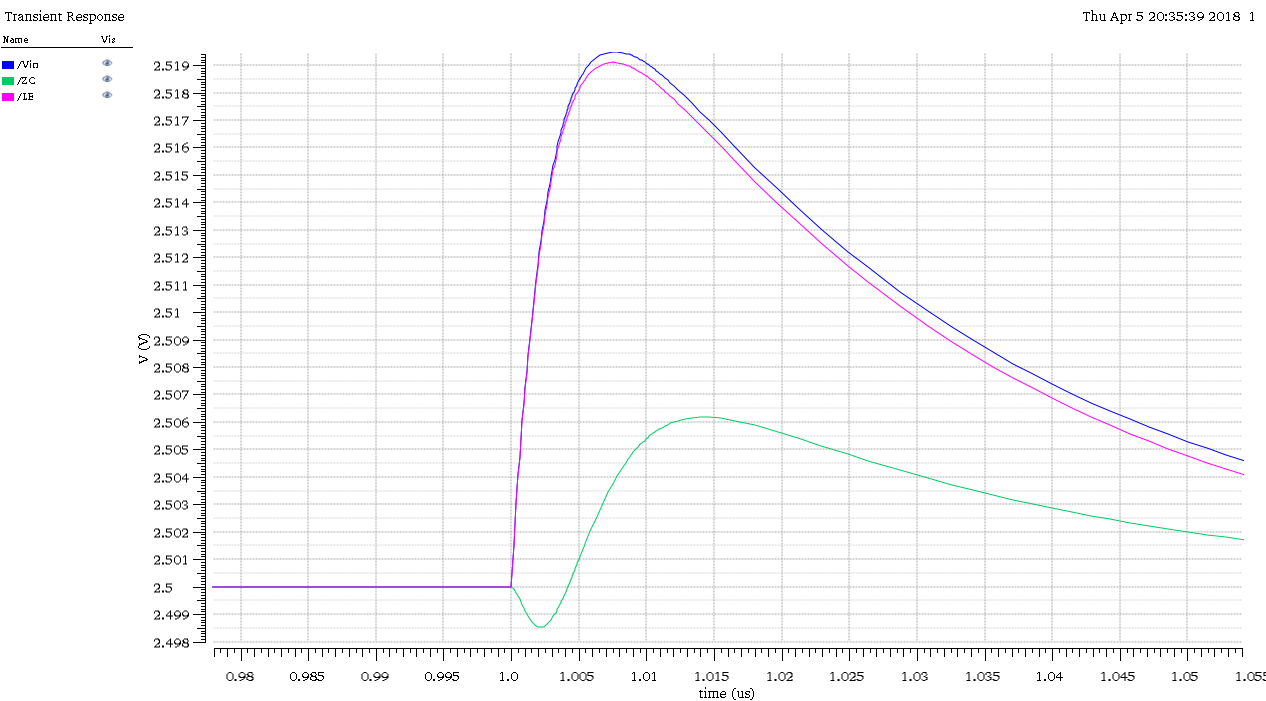
\includegraphics[scale=.40,keepaspectratio=true]{images/nowlin_out.png} 
\caption{Nowlin differential (green) and high pass filtered (blue) outputs in response to 3 ns 20 mV pulse (purple). }
\label{fig:nowlinout}
\end{figure}
\subsection{Zero Crossing Discriminator Stage}
\par The differential outputs of the Nowlin circuit are used as inputs to a zero crossing discriminator. This discriminator is created by cascading three differential amplifiers together and connecting the final output to a high speed comparator. This circuit will provide a digital output that is a logic high (5V) when the two differential output voltages cross the 0V threshold when referenced to analog ground (\emph{AGND}). This will allow the circuit to produce an output independent of the input pulse amplitude \cite{CFD}. 
\par To achieve amplitude independence it is important that the delay time set in the Nowlin circuit is optimal. With a short delay time there is very little under drive in the output of the final differential amplifier which could prevent the comparator from firing. The importance of this underdrive voltage is illustrated in Figure~\ref{fig:underdrive}. With too much delay there is not enough slew rate to accommodate the fast timings that are needed (1 ns or less time walk and jitter). The importance of high slew rate is the reason fro cascading multiple differential amplifiers as opposed to using one high gain diff-amp. The amplifiers designed have a gain of ~5. For first order approximations it is known that the bandwidth of a differential amplifier obeys Eqn~\ref{eq:bw} \cite{CFD}.
\begin{eqnarray}
BW = \frac{0.35}{t_{10-90}}
\label{eq:bw}
\end{eqnarray}
\begin{figure}[ht]
\centering
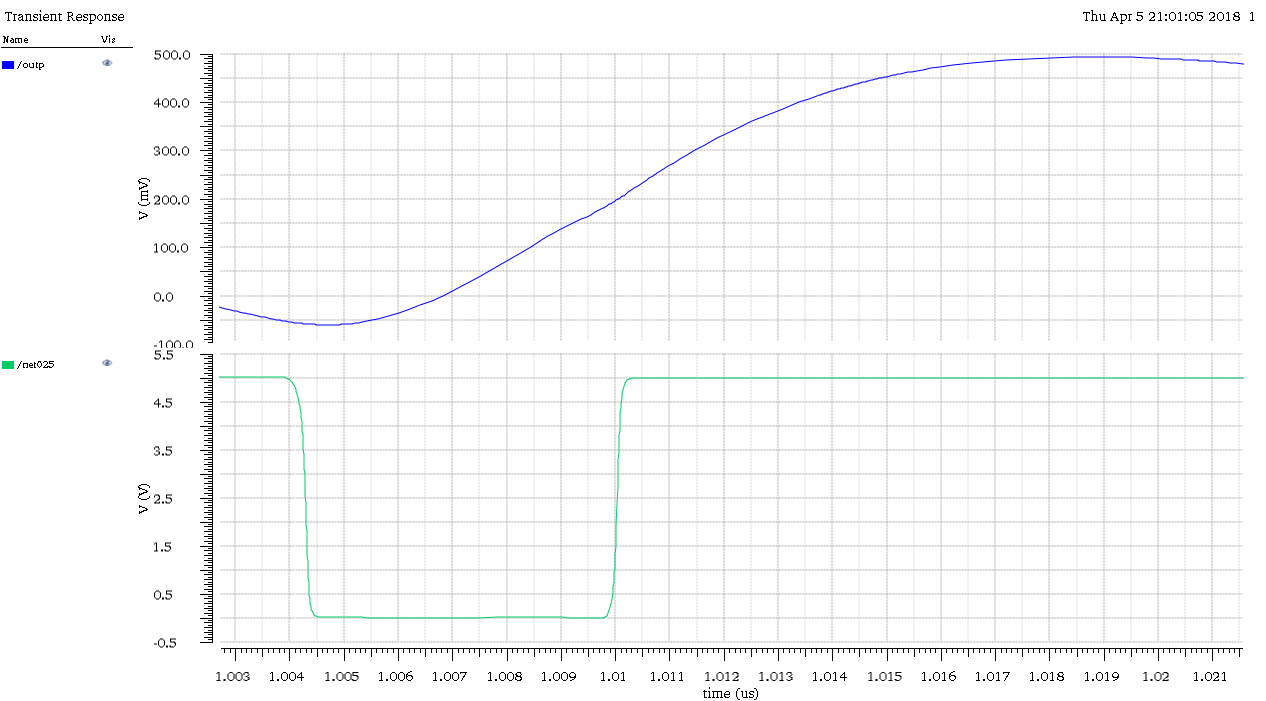
\includegraphics[scale=.4,keepaspectratio=true]{images/zcd_out.png} 
\caption{Zero crossing discriminator comparator output showing underdrive to force output low.}
\label{fig:ZCD}
\end{figure}

\par The zero crossing discriminator needs an overall bandwidth of 50 Mhz. Since there are three diff-amp stages, each diff-amp needs a total bandwidth of $\sqrt{3} \approx 1.7$  times larger. This means the differential amplifiers needs a bandwidth of at least 85 Mhz in order for the zero cross discriminator to function properly. The final output of the comparator is delayed by 10 nsec in order to ensure the leading edge discriminator output fires first.\newpage
\begin{figure}[ht]
\centering
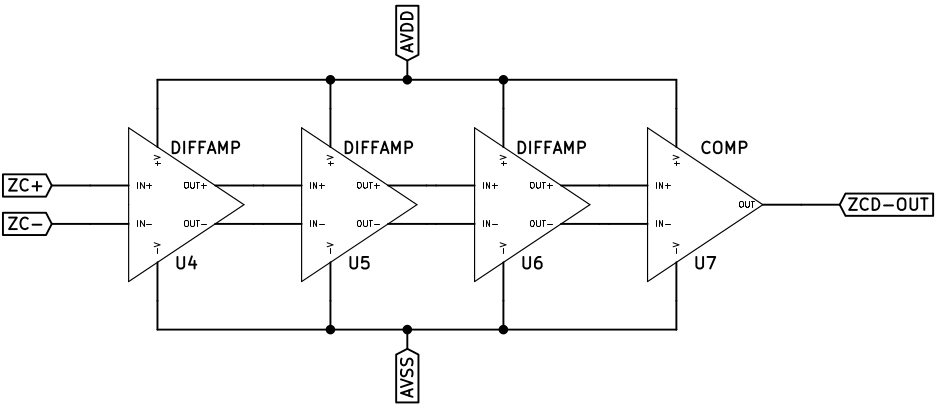
\includegraphics[scale=.55,keepaspectratio=true]{images/zcd_circuit.png} 
\caption{Zero crossing discriminator stage.}
\label{fig:ZCD}
\end{figure}
\subsection{Leading Edge Discriminator Stage}
\par The high pass filter output of the Nowlin is used as a input to a leading edge discriminator. This discriminator is comprised of a differential amplifier that connects to a differential to single ended amplifier with a gain of ~1. The differential amplifier helps remove common mode noise \cite{COMMON_MODE}. Removing noise is essential to improving the jitter as it is directly related to the input noise  as shown by Eqn~\ref{eq:jitter} \cite{CFD}. 
\begin{eqnarray}
\sigma _t  = \frac{\sigma _v}{SR}
\label{eq:jitter}
\end{eqnarray}
\par The output of the differential to single ended amplifier is compared against a user set threshold voltage that is generated by a 6-bit DAC. The DAC is used to set the noise floor threshold to give even greater noise immunity, as well as help nullify effects from offset voltages in the amplifier stages. Since the CFD channel can operate regardless of input voltage polarity, this DAC has a negative polarity control signal that when enabled (ie. 5V) will provide an output voltage that is below \emph{AGND}. The same diff-amp and comparator circuits from the zero crossing discriminator circuit are used in the leading edge discriminator as well. 

\par The DAC threshold voltage will be configured based on the noise floor and the expected input pulse amplitude for the experiment. Once an input pulse arrives from the Nowlin circuit and rises above this threshold voltage the leading edge discriminator will fire a digital  output pulse (5V). This output pulse indicates that an input pulse has arrived so that further output from the zero crossing discriminator can be treated as valid. Figure~\ref{fig:ledout} shows the output generation of the leading edge discriminator.
\begin{figure}[ht]
\centering
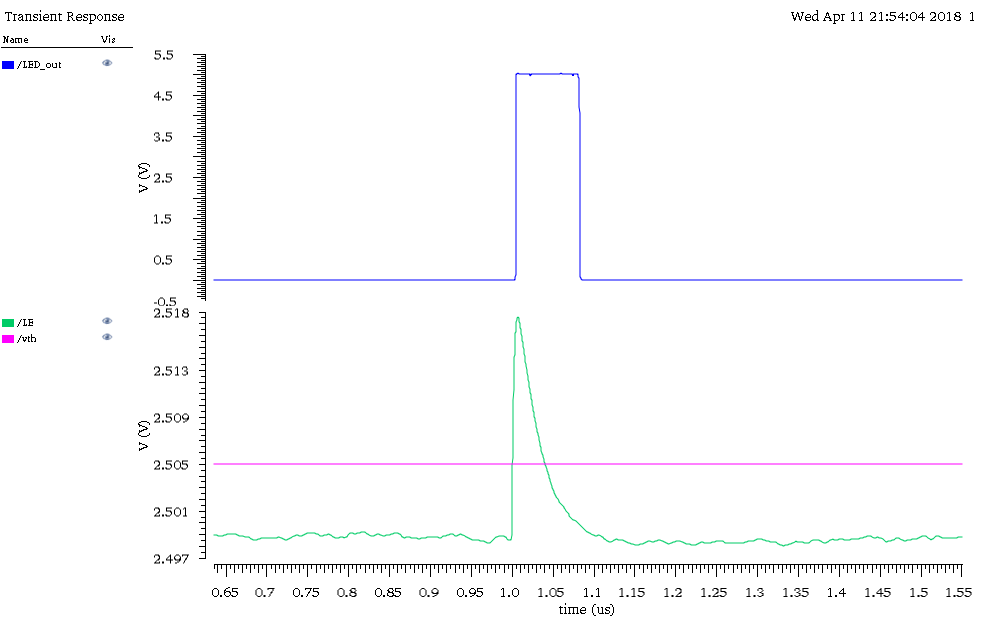
\includegraphics[scale=.4,keepaspectratio=true]{data/led_noise.png} 
\caption{Leading edge discriminator output generation showing noise immunity.}
\label{fig:ledout}
\end{figure}
\begin{figure}[ht]
\centering
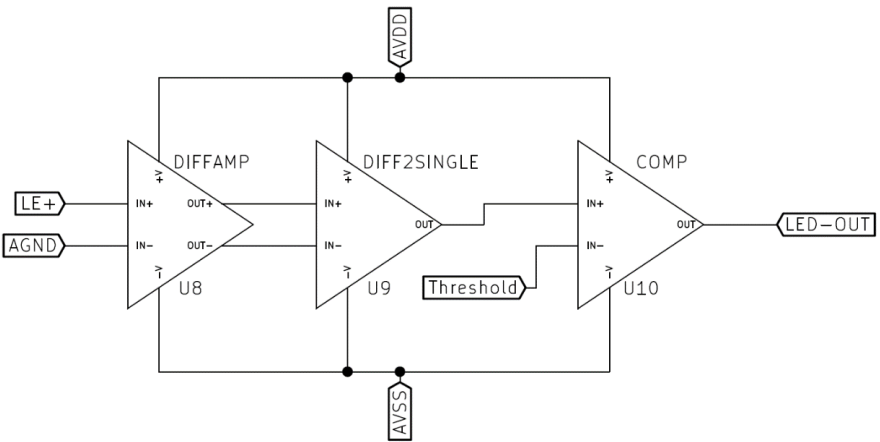
\includegraphics[scale=.5,keepaspectratio=true]{images/led_circuit.png} 
\caption{Leading edge discriminator stage.}
\label{fig:LED}
\end{figure}
\subsection{Oneshot Stage}
\par The timing pulse of each CFD channel is produced in the oneshot stage (Fig~\ref{fig:oneshot-stage}). This stage contains and edge detector, two oneshot circuits, and a 2-bit unipolar DAC. The input to the oneshot stage comes from the digital output pulses from the comparators in both the leading edge discriminator and zero crossing discriminator. 
\par The outputs of the two dicriminator stages are first ANDed together. Since the zero crossing discriminator (ZCD) stage is delayed, the leading edge discriminator stage (LED) can be used as a qualifier. The AND of these two thus guarantees that the output of the ZCD is from a real input pulse and not random transients. This qualification pulse is shown in Figure~\ref{fig:qualifier}. The ANDed discriminator signals are then used as input to an edge detector whose output triggers a oneshot circuit.
\begin{figure}[ht]
\centering
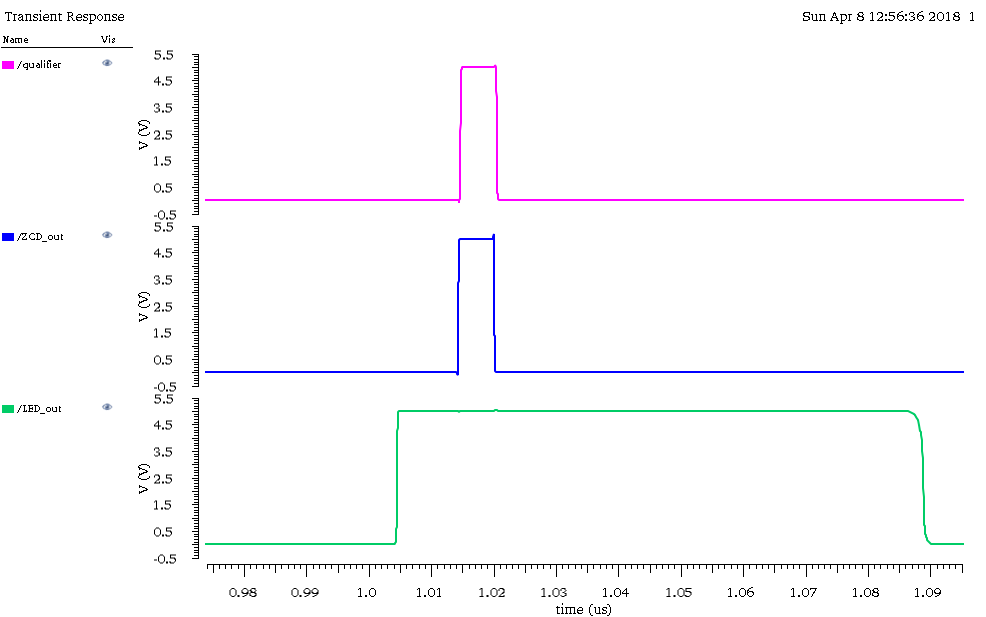
\includegraphics[scale=.4,keepaspectratio=true]{images/qualifier.png} 
\caption{Leading edge and zero cross discriminator outputs generating qualifier pulse for oneshot.}
\label{fig:qualifier}
\end{figure}
\par A oneshot circuit is a circuit whose input is a narrow pulse and outputs a fixed width pulse \cite{ONESHOT}. There are two oneshots in this stage. The first one creates the timing pulse that will eventually be output to the CFD16C output pad for the channel. The second oneshot is triggered by the first, and creates a lockout timing pulse to prevent the first oneshot from firing for a fixed amount of time. The width of the timing pulse is determined by a 2-bit logarithmically distributed digital-to-analog converter (DAC) with timing values shown in Table~\ref{Tab:oneshot-pw}. The lockout oneshot has its pulse width determined by an analog control voltage that is generated off chip.
\begin{figure}[ht]
\centering
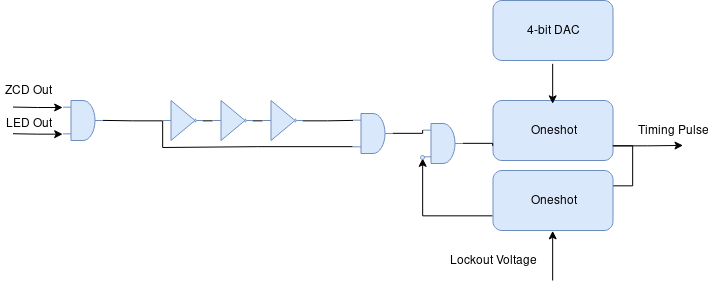
\includegraphics[scale=.6,keepaspectratio=true]{images/oneshot_stage.png} 
\caption{Oneshot stage.}
\label{fig:oneshot-stage}
\end{figure}
\begin{table}[ht]
\centering
	\begin{tabular}{|l|p{4cm}|}
		\hline
		Digital Value & Pulse Width (nsec)\\\hline
		0 & 500\\\hline
		1 & 250\\\hline
		2 & 100\\\hline
		3 & 50\\\hline
	\end{tabular}
    \caption{DAC digital code word to oneshot pulse width mapping.}
 	\label{Tab:oneshot-pw}
\end{table}
\subsection{Output Stage}
\begin{figure}[ht]
\centering
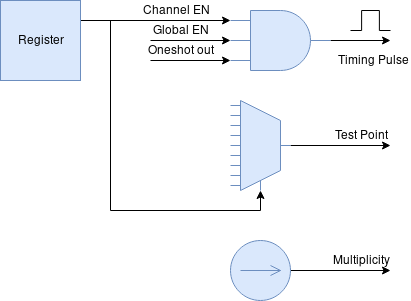
\includegraphics[scale=.6,keepaspectratio=true]{images/output_stage.png} 
\caption{Output generation stage overview.}
\label{fig:output-stage}
\end{figure}
\par All of the channel outputs are generated in a final output stage that contains a configuration register and an analog mutliplexer. Each channel has three outputs that are generated: the timing pulse output which connects to an output pad, a multiplicity current that goes to a resistor in the common channel, and a test point output.
\par The timing pulse output comes from the output oneshot in the oneshot stage but is qualified in this stage. The output timing pulse will only be seen on the output pad of the channel if the global enable pin and the channel enable control signal are held in a logic high (5V). The global enable signal comes from a pin connection on the chip package while the channel enable is produced by the configuration register in the output stage.
\par The multiplicity current is generated by a current mirror. There are two bias currents that are provided to each channel: one that is proportional to absolute temperature (PTAT) and one that has a zero temperature coefficient (ZTC). The PTAT current is copied to the output stage and controlled with a PFET switch. This current, when enabled, is sent to the common channel here it is connected to a resistor to ground (\emph{AVSS}). Thus the more currents that are enabled, the larger the voltage across this resistor, creating a proportional voltage to the number of channels that have fired.
\par The global channel OR output is also generated in the common channel. This logical OR signal is achieved by using a pseudo NMOS NOR gate. One NFET is placed in the output stage of each channel with a single PFET in the common area, followed by an inverter. This circuit is described further in Chapter 3.
\par A test point output is also provided by the output stage. This test point will allow a user to route several analog nodes from within to the channel to a test point pad on the chip. An analog multiplexer is used to select from these possible test points. The register in the output stage contains the selection bits for this multiplexer, as well as a bit for the channel enable signal. Figure~\ref{fig:output-stage} shows the overall structure of the output stage. Table~\ref{tab:outreg} shows the bit configurations for the output stage register, and Table~\ref{tab:tpval} shows the possible test point values.

\begin{table}[ht]
\centering
	\begin{tabular}{|l|p{3cm}|}
		\hline
		Bit Position & Purpose\\\hline
		0-3 & Select TP node.\\\hline
		4 & Channel EN.\\\hline
	\end{tabular}
    \caption{Register bit functionality.}
 	\label{tab:outreg}
 	\end{table}
 	\begin{table}[ht]
 	\centering
	\begin{tabular}{|l|p{7cm}|}
		\hline
		Select Value & Test Point\\\hline
		0 & AGND\\\hline
		1 & 2-bit DAC CV\\\hline
		2 & Nowlin high pass filter output\\\hline
		3 & 6-bit DAC output\\\hline
		4 & Differential to single ended amp output.\\\hline
		5 & Bandgap voltage\\\hline
		6 & Nowlin constant fraction output\\\hline
		7 & Nowlin delayed output\\\hline
	\end{tabular}
    \caption{Available test points from the AMUX.}
 	\label{tab:tpval}
\end{table}
%Table from image: 

%\begin{table}[htbp!]
% \centering
 %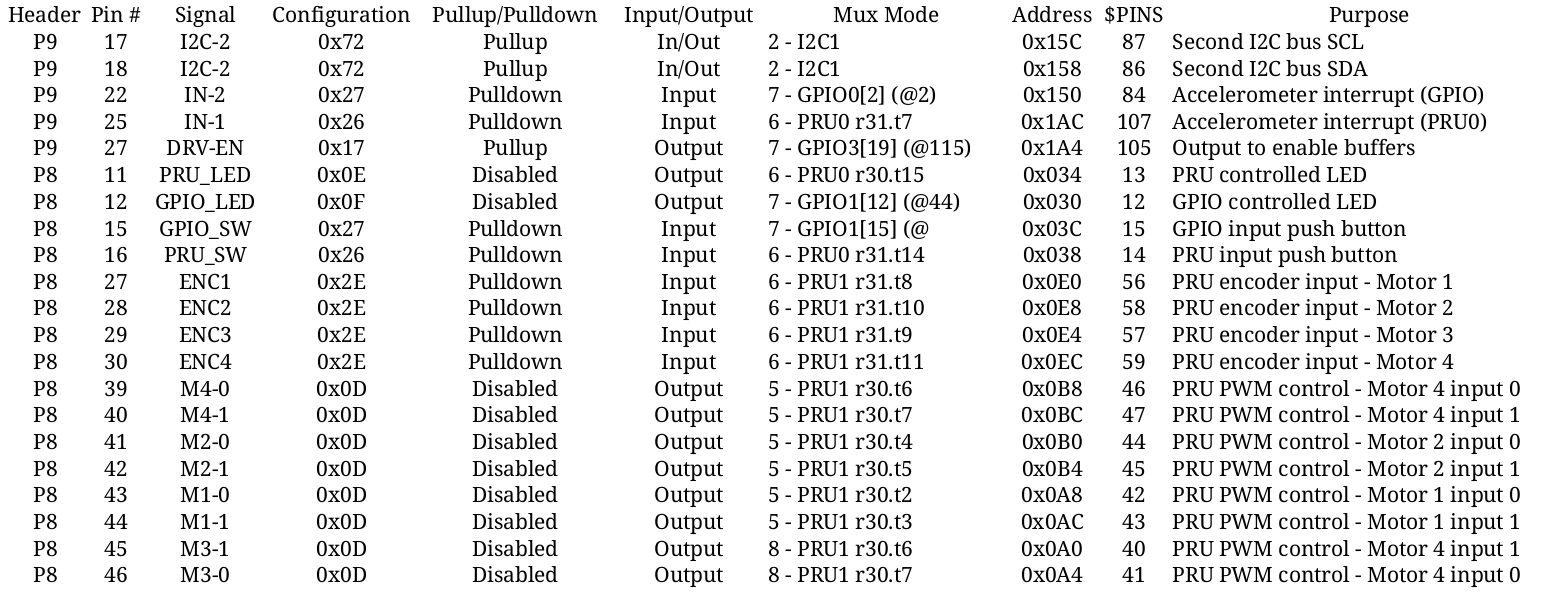
\includegraphics[scale=.3,keepaspectratio=true]{./images/Pinlist.png}
 %\caption{BeagleBone Black Pins Used by SIpeUE Robot Cape}
 %\label{tab:Pin_list}
%\end{table}

\chapter{CIRCUIT LEVEL DESIGN}
\par The CFD16C contains 16 CFD channels and one common channel. The single common channel contains configuration and biasing circuitry for the other 16 channels to operate correctly. Some of the designs from the PSD8C microchip have been reused in the CFD16C design. The CFD16C is being designed in the AMIS 0.5 micron process. This is a three metal process that supports double poly capacitors, and high resistance poly layers. 
\section{Process Parameters}
\par The process parameters for the CMOS devices in the AMIS 0.5 micron process is shown below. All process parameters listed are nominal values only.

\begin{itemize}
\item
Threshold voltage (V$_{tn}$) of NFET devices is 0.75 V.
\item
Threshold voltage (V$_{tp}$) of PFET devices is -1 V.
\item
Transconductance parameter (K$_{pn}$) of NFET devices is 100 $\frac{\mu A}{V^{2}}$.
\item
Transconductance parameter (K$_{pp}$) of PFET devices is 32 $\frac{\mu A}{V^{2}}$.
\item
The $\frac{1}{f}$ noise parameter (K$_{an}$) of NFET devices is $6.3\cdot10^{-26}$ A F.
\item
The $\frac{1}{f}$ noise parameter (K$_{ap}$) of PFET devices is $3.8\cdot10^{-30}$ A F.
\end{itemize}

\section{Common Channel}
\par The common channel contains circuitry used by all 16 CFD channels. There is a bandgap voltage reference that was reused from the PSD8C design, a common source amplifier to buffer the multiplicity output, configuration registers, and current replicator circuitry to generate bias currents for each channel. 

\subsection{Digital Configuration}
\par The digital configuration circuitry was all custom designed for the CFD16C. The configuration logic is made up of a D-latch scan chain with decoding logic for the address and mode bits. The D-latches are parallel loaded on the rising edge of \emph{STB} if the \emph{ADDR} and \emph{MODE} busses match the hard coded values for the configuration register. Once the D-latches are loaded, the scan logic allows the data from all registers to be read out using a two phase non-overlapping clock (\emph{SI\_CLK} \& \emph{SO\_CLK}). 
\par The most significant bit of the \emph{MODE} bus allows all registers whose mode is selected to be configured at once. With this bit set, \emph{ADDR} is ignored and the lower three \emph{MODE} bits are used to select a specific register in the channels. The register matching this mode in \emph{all} channels is then loaded with data on the positive edge of \emph{STB}.
\subsection{Bandgap Reference}
\par The bandgap voltage reference used in this design was copied from PSD8C as a known working solution. A bandgap voltage reference is used to provide a 1.23 V reference point that is independent of temperature or power supply noise \cite{BANDGAP}. The bandgap voltage is created by generating a PTAT current of $\approx 120 \mu A$ through a series resistor and a diode-connected parasitic bipolar PNP transistor \cite{ALLEN-HOLBERG}. The PTAT current has a positive temperature coefficient while the PNP transistor has a negative temperature coefficient of $\approx -2 \frac{mV}{C}$ for its base-emitter voltage creating a nodal voltage with no temperature dependence.
\par This bandgap topology produces an output voltage of $\approx 1.2 V$ with near zero temperature independence. The design has been used in the PSD8C and HINP16C microchips and has shown good performance so the design was reused and remains unmodified. Additional information on this bandgap circuit design can be found in \cite{HINP-THESIS}.
\subsection{Bias Currents}
\par Two bias currents are generated for use in the CFD channels. A current that is proportional to absolute temperature (PTAT) and one that has zero temperature coefficient (ZTC). The bandgap circuit from PSD8C alread creates a 120 $\mu$A PTAT current so this current can be replicated for each channel using 16 current mirrors \cite{PROCTOR}. This PTAT current is used in the differential amplifiers, which are actually operational transconductance amplifiers (OTAs). A weakly or moderately inverted FET has a tranconductance linearly proportional to bias current but inversely proportional to absolute temperature. Thus by using PTAT currents for the moderately inverted FETs in the OTA design the transconductance of the FETs becomes independent of temperature \cite{TRANS}.
\par Having tranconductance, or g$_{m}$, independent of temperature is important for the design of the CFD16C since the GBW of the ZCD diffamp stages is dependent on the g$_{m}$ of the devices. Having no temperature dependence on g$_{m}$ means the ZCD and LED stages will function the same regardless of the temperature. 
\par The ZTC current was generated using an opamp circuit shown in Figure~\ref{fig:ztc}. In this circuit, the temperature independent bandgap voltage is applied to the inverting terminal of an opamp. The output of the opamp connects to the gate of a PFET whose drain is connected to a zero temperature coefficient 100 k$\Omega$ resistor. A feedback connection to the non-inverting terminal of the opamp is made to the drain of the PFET as well. 
\begin{figure}[htbp!]
\centering
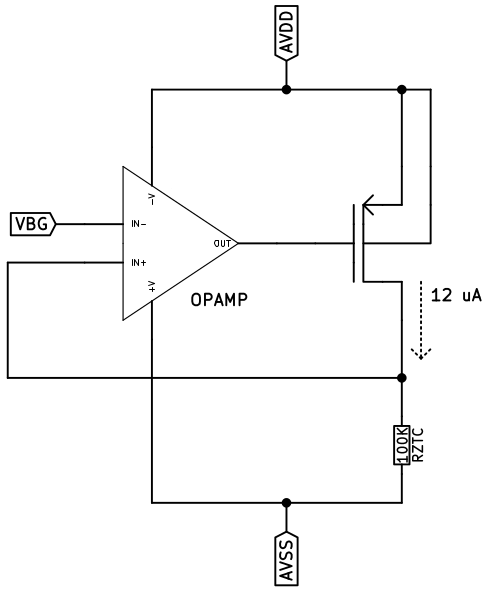
\includegraphics[scale=.45,keepaspectratio=true]{images/ztc_gen.png} 
\caption{Zero temperature coefficient current generator.}
\label{fig:ztc}
\end{figure}
\par The ZTC resistor is made from a resistor with positive temperature coefficient (NY), and one that has a negative temperature coefficient (HY). The ratio to achieve temperature independence in this process is $\approx$ 0.7 NY to 0.3 HY. Since a 12 $\mu$A ZTC current is desired, a 100 k$\Omega$ resistor was made using a 70 k$\Omega$ NY resistor and a 30 k$\Omega$ HY resistor. This ZTC current is replicated using 16 current mirrors to provide one for each channel. The ZTC currents are used to give the DAC circuits an output that doesnt depend on temperature. 
\section{Nowlin Circuit}
\par The Nowlin circuit is used at the input stage of each of the CFD channels and is shown in Figure~\ref{fig:Nowlin}. The Nowlin circuit turns a single ended input pulse into a differential signal for use in the zero crossing discriminator. This is achieved by taking a constant fraction of the input voltage using a resistor voltage divider (ZC-). The ratio in this case is $\frac{2}{3}$ or $\approx 0.67$. The other leg (ZC+) of the differential output is a delayed version of the input pulse. The delay comes from resistor R3 in Figure~\ref{fig:Nowlin} and the programmable capacitor C1. This creates a configurable RC time constant to delay the input signal. 
\begin{figure}[ht]
\centering
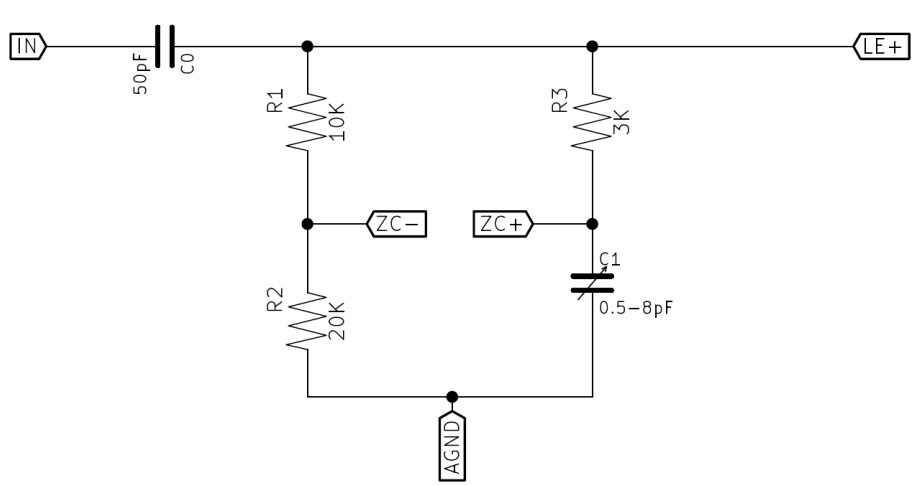
\includegraphics[scale=.6,keepaspectratio=true]{images/nowlin_circuit.png} 
\caption{Nowlin circuit.}
\label{fig:Nowlin}
\end{figure}
\par C0 and the series combination of R1 and R2 create a high pass filter whose output is called LE+. The corner frequency of this high pass filter is given by Eqn~\ref{eq:hpf}. This high pass filter output is used as input the the leading edge discriminator. The reason for high pass filtering is to remove any low frequency and DC noise present on the input pin as the actual signal pulse will always be a high frequency exponential pulse.
\begin{align}
f_{c} = \frac{1}{2\pi \cdot(R1+R2)\cdot C1} &\approx 100 kHz
\label{eq:hpf}
\end{align}
\par The programmable capacitor (Figure~\ref{fig:pcap}) in the Nowlin circuit is created by using switches, in this case transmission gates, to connect individual capacitors in and out of circuit with the Nowlin. Two transmission gates (t-gates) per capacitor are used to accomplish this. The two t-gates are connected in series which creates a circuit with three nodes: left, middle, right. The left node connects to the top plate of a 0.5 pF capacitor that is always in circuit, referenced to \emph{AGND}. The middle node connects to the top plate of one of the programmable capacitor elements, which is also referenced to \emph{AGND}. The right node of the switch circuit connects to \emph{AGND}.
\par In this configuration when the control signal is on (ie. 5V), the capacitor at the middle node connects in parallel with the 0.5 pF capacitor, adding more capacitance to the ZC+ node in the Nowlin. If the control signal is off (ie. 0V) then the capacitor is shorted out to \emph{AGND} discharging it and removing capacitance from the ZC+ node. In total there are four of these capacitor circuits, one for each bit of the programmable capacitor bus. Each capacitor is binary weighted with the following values: 0.5 pF, 1 pF, 2 pF, and 4 pF. This gives a total in circuit capacitance of 8 pF and a minimum in circuit capacitance of 0.5 pF. Table~\ref{tab:pcap} shows the bit order of these capacitor elements. Referencing this table shows that the total capacitance at the ZC+ node will be $C_{total} = D \cdot 0.5pF + 0.5pF$ where D is the decimal value of the 4-bit programmable capacitor bus.
\begin{table}[ht]
\centering
	\begin{tabular}{|l|p{4cm}|}
		\hline
		Bit Mask & Capacitor Value\\\hline
		0001 & 0.5 pF\\\hline
		0010 & 1 pF\\\hline
		0100 & 2 pF\\\hline
		1000 & 4 pF\\\hline
	\end{tabular}
    \caption{Programmable capacitor bit position values}
 	\label{tab:pcap}
\end{table}
\begin{figure}[ht]
\centering
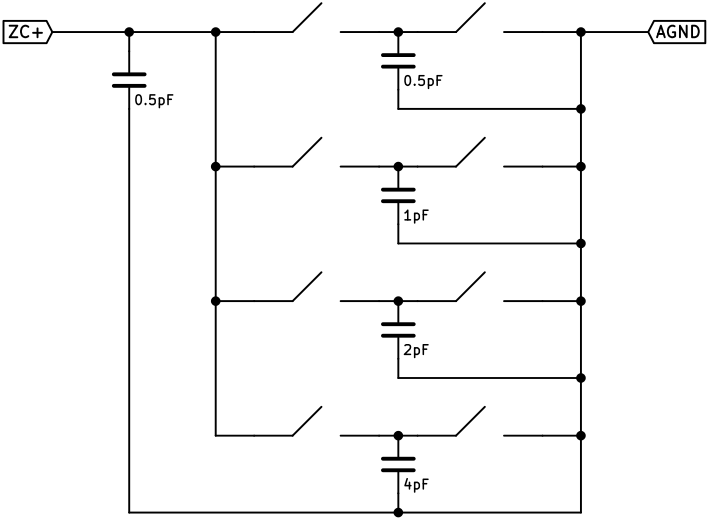
\includegraphics[scale=.6,keepaspectratio=true]{images/pcap_circuit.png} 
\caption{Programmable capacitor circuit.}
\label{fig:pcap}
\end{figure}
\section{Differential Amplifier}
\par The most critical piece of the zero crossing discriminator is the differential amplifier used to gain up the differential signal from the Nowlin and enhance the slew rate. The differential amplifier is a fully differential OTA to give better common mode rejection ratio that a single output amplifier. The OTA is biased with a PTAT current of 325 $\mu$A that combines with a diode connected NFET to create a voltage of $\approx 1.1$ V for biasing current mirrors in the circuit.
\par Figure~\ref{fig:diffamp} shows the OTA circuit in it's entirety. The OTA is composed of two biasing NFETs (M5 \& M9) whose gates connect to the 1.1 V bias transistor, and a diode connected PFET (M8) for biasing the differential pair. The input is applied to the differential pair (M1 \& M2) that is loaded with diode connected PFETs (M3 \& M4). The gain is then determined by the ratio of transconductance (g$_{m}$) of the differential pair transistors and their diode connected transistor load, giving a gain of $\approx 2$ (6 dB) \cite{ALLEN-HOLBERG}. The differential amplifier has a bandwidth of $\approx 310$ MHz with a slew rate of $\approx 150$ $\frac{V}{\mu sec}$. 
\begin{figure}[htbp!]
\centering
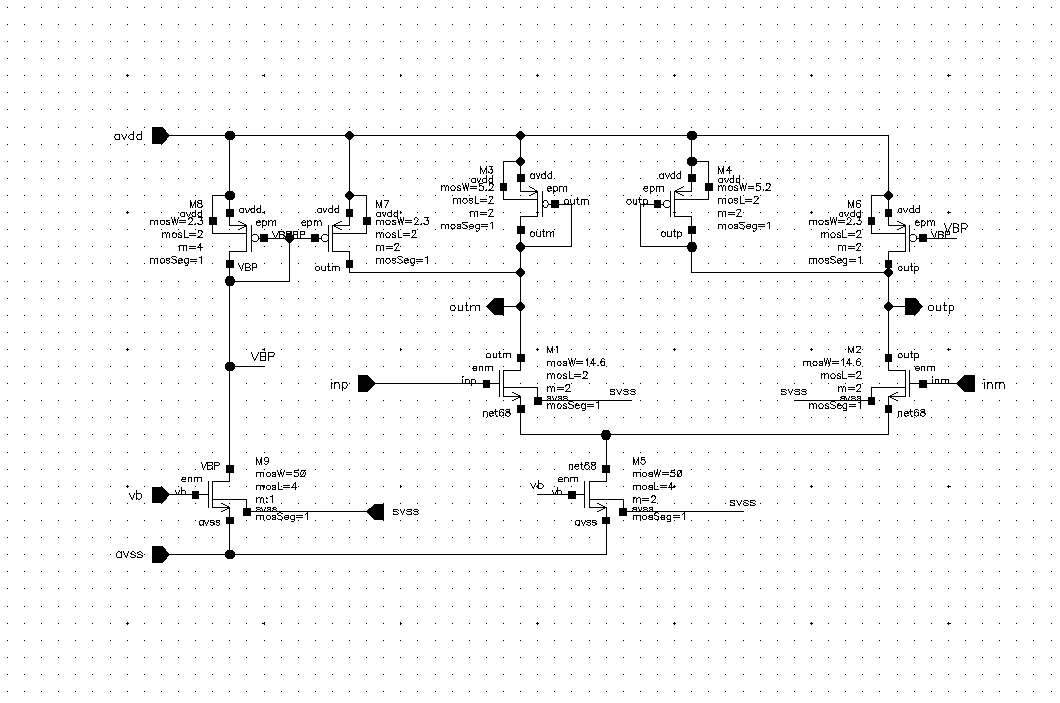
\includegraphics[scale=.45,keepaspectratio=true]{images/diffamp.png} 
\caption{Differential amplifier circuit.}
\label{fig:diffamp}
\end{figure}
\section{Comparator}
\par A high speed analog comparator is needed in both discriminator stages to produce the digital output pulses needed for the output timing pulse generation. An analog comparator will output a logic high (5V) when the noninverting input is larger than the inverting input.  Typically a comparator has a large positive feedback stage in the form of cross coupled NFETs \cite{BAKER}. Because of systematic offset voltage in the transistors of the diffamp stages, this large positive feedback would cause the comparator output to latch to one of the supply rail voltages. Instead, a fully differential self biasing comparator design was used. This design gives equal slew rate in both the negative and positive directions but uses more transistors \cite{ALLEN-HOLBERG}. 
\par A differential pair (MN18 \& MN19) acts as the input to the comparator circuit. A self biasing network (MP9, MP10, \& MN20) allow the swing of the comparator output to be equal in both directions. The output of the comparator is then buffered by three large inverter stages to give a rail to rail digital output signal with an extremely fast output rise time of $\approx 200$ psec. 
\begin{figure}[htbp!]
\centering
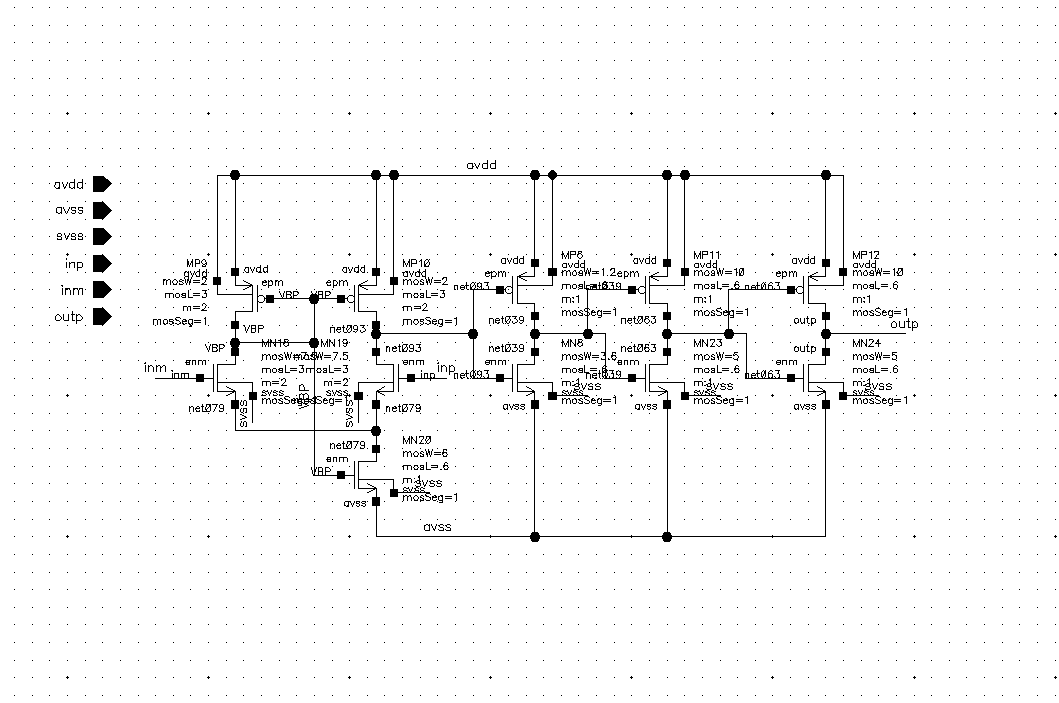
\includegraphics[scale=.55,keepaspectratio=true]{images/comp.png} 
\caption{Comparator circuit.}
\label{fig:comp}
\end{figure}
\section{Oneshot DAC}
\par The oneshot circuit needs an analog control voltage to set the pulse width of the output timing pulse. The accuracy of the pulse width is not as important as the ability to have four logarithmically distributed pulse widths, so a simpler DAC solution was used. This DAC consists of an opamp voltage doubler that takes the bandgap voltage and doubles it to $\approx 2.5$ V. This voltage is applied to the top of a string of series resistors that act as voltage dividers, creating four voltage outputs. These outputs connect to transmission gates that allow a specific node to be selected and routed to the output of the DAC. Table~\ref{tab:dac} shows the nodal voltages that can be added to the output with each bit of the DAC.
\begin{table}[ht]
\centering
	\begin{tabular}{|l|p{4cm}|}
		\hline
		Digital code & Output Voltage\\\hline
		00 & 1.1 V\\\hline
		01 & 1.5 V\\\hline
		10 & 2 V\\\hline
		11 & 2.5 V\\\hline
	\end{tabular}
    \caption{Oneshot DAC bit voltages.}
 	\label{tab:dac}
\end{table}

\section{Oneshot Circuit}
\par The oneshot circuit used in CFD16C was a design borrowed from the PSD8C. The oneshot circuit uses an SR latch and a Schmitt trigger with a delay circuit on its input. The input edge is applied to the S input of the SR latch causing the output to go high. This SR latch output is the output of the oneshot circuit. A high output on the SR latch causes a 400 fF capacitor on the input of the Schmitt trigger to lower, which eventually causes the Schmitt trigger to fire. The output of the Schmitt trigger connects to the R input of the SR latch, causing the output to go low. The width of this output pulse is determined by a bias current created by diode connected transistors and current mirrors. The otuput pulse width can thus be calculated by Eqn~\ref{eq:oneshot} 
\begin{align}
t_{pulse} = \frac{C \cdot \Delta V_{c}}{I_{bias}}
\label{eq:oneshot}
\end{align}
where $\Delta V$ is the change in voltage of the capacitor before the Schmitt trigger fires and I$_{bias}$ is the bias current created from the biasing circuit. The Schmitt trigger fires when the capacitor voltage drops below 1.5 V. This rate at which $\Delta V$ changes can be configured by changing the bias voltage applied to a diode connected NFET, which in turn changes I$_{bias}$.
\section{Output Generation}
\par Each channel has several outputs that either connect directly to pads on the chip package or be routed to the common channel. All channel outputs are created in a dedicated output stage. The timing pulse is qualified here before going off chip, the global channel OR, test point, and a multiplicity current are also generated here before being routed to the common channel.
\subsection{Multiplicity}
\par Each channel outputs a single PTAT current for generation of a multiplicity output. The current is controlled by a PFET switch to allow current to flow only when the timing pulse output is high. This 12 $\mu$A current is combined with a resistor and common source amplifier in the common channel. The output of the common source amplifier is connected to the output pad and will have an output range between 1 V (no current) and 3V (192 $\mu$A) by using a 10K$\Omega$ resistor to turn the channel multiplicity currents into a voltage. This gives an analog voltage proportional to the number of channels that have fired. 

\subsection{Channel OR}
\par A global channel OR is created by using pseudo NMOS logic to create an OR gate that is globally distributed among all 16 channels \cite{NMOS}.  In each channel there is a single NFET whose gate is connected to the output timing pulse. The source of this NFET is connected to \emph{AVSS} while the drain connection is routed to the common channel. A single PFET is located in the common area, with its gate connected to \emph{AVSS}. The drain of all of the channel NFETs connect to the drain of he PFET creating a globally distributed pseudo NMOS NOR gate. The output of this gate is connected to a CMOS inverter to create an OR gate whose output will be high if any one of the channels fires.

\subsection{Timing Pulse}
\par The output timing pulse is qualified in this stage. In order to trigger the mulitplicity current, global channel OR, or show up on the output pad the channel enable and global enable signals must be present. This qualification logic is shown in Figure~\ref{fig:output}.
\begin{figure}[htbp!]
\centering
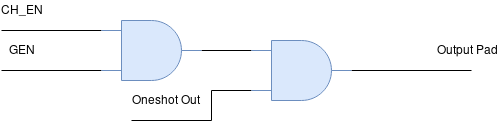
\includegraphics[scale=.55,keepaspectratio=true]{images/output.png} 
\caption{Output timing pulse qualification.}
\label{fig:output}
\end{figure}

\chapter{SIMULATION}
\section{Methods}
\par This chapter presents simulated data for many of the circuits designed for the CFD16C. This data was acquired using the Spectre simulator with Verilog-A test bench fixtures that produced stimuli for circuit level devices. The data presented represents ideal circumstances. The CFD16C is being migrated over to a different design process detailed in Chapter 5 and thus only circuits that were completed and simulated in the 0.5 micron AMIS process will be detailed in this chapter.

\section{Common Channel}
\par Most of the completed circuits from the common channel were borrowed from HINP16C or PSD8C, including the bandgap and bias current generators. The configuration registers and address logic were created and tested by another graduate student, Pohan Wang, as part of a masters project and proved to work well. 

\subsection{Bandgap}
\par The Bandgap reference design was reused from PSD8C, which in turn borrowed the design from HINP16C. This bandgap has a very stable 1.2 V output with little temperature dependence. The design has been used several times and proven to function very well. More details about this circuit can be found in \cite{HINP-THESIS}.

\subsection{Bias Current Generators}
\par Both the PTAT and ZTC bias current generators were designs borrowed from HINP16C with no modifications. Detailed performance characteristics for these designs can be found in the HINP16C documentation \cite{HINP-THESIS}.

\section{Oneshot DAC}
\par It is important that the oneshot output pulse width not be affected by temperature. For this reason the temperature independence of the oneshot DAC is very important. The DAC was simulated with temperature ranges between -10 $^{\circ}$C to 90 $^{\circ}$C as shown in Figure~\ref{fig:dactemp}. The output voltage shows a temperature coefficient of $\approx$ -7 $\frac{\mu V}{^{\circ}C}$.
\begin{figure}[htbp!]
\centering
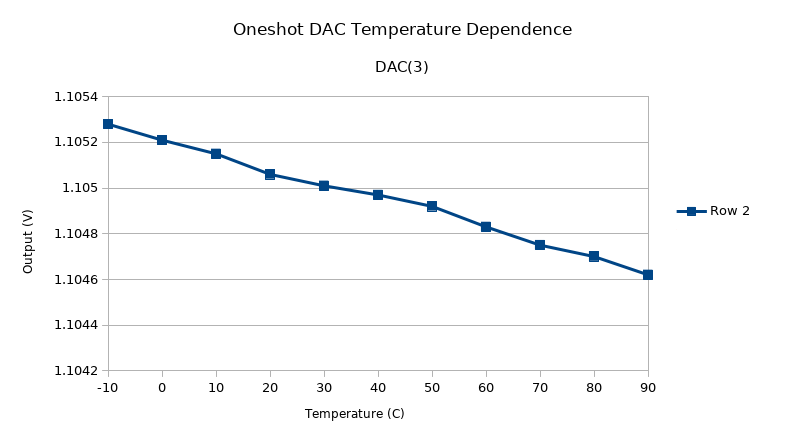
\includegraphics[scale=.55,keepaspectratio=true]{data/dac_temp.png}
\caption{Oneshot DAC temperature dependence.}
\label{fig:dactemp}
\end{figure}
\section{Oneshot}
\par The oneshot circuit is borrowed from HINP16C and was also used in PSD8C. The circuit has been proven to work well, allowing for controllable output pulse widths between 50 nsec and 500 nsec. More detailed analysis is available in the HINP16C documentation \cite{HINP-THESIS}.

\section{Nowlin}
%TODO: Nowlin filter attenuation
% Nowlin outputs for 3 nsec and 100 nsec, +/- 20 mV and +/- 2 V signals
\par The Nowlin circuit contains a high pass filter to help remove low frequency noise before an input pulse is sent to the LED. This allows the LED to fire only in response to a real input pulse and not transient noise. The input signal pulse comes in the form of on exponential rise and decay in voltage and can have rise times between 3 nsec and 100 nsec, and fall times between 30 nsec and 1 $\mu$sec. This is a wide operating range so filter attenuation can be a concern. A high pass filter attenuates signals according to Eqn~\ref{eq:atten} where X$_{C}$ is the capacitor reactance \cite{CIRCUITS}.
\begin{align}
A_{v} = \frac{R}{\sqrt{R^{2} \cdot X_{C}^{2}}}
\label{eq:atten}
\end{align}
\par Figures~\ref{fig:atten3}-\ref{fig:atten100} show the attenuation of this high pass filter for both a 3 nsec and 100 nsec input pulse. The 3 nsec pulse is attenuated by $\approx$ 3\% of the original input signal, while the 100 nsec pulse is attenuated by $\approx$ 10\%. Both of these results are well within the acceptable range for the CFD channel to function appropriately.
\begin{figure}[htbp!]
\centering
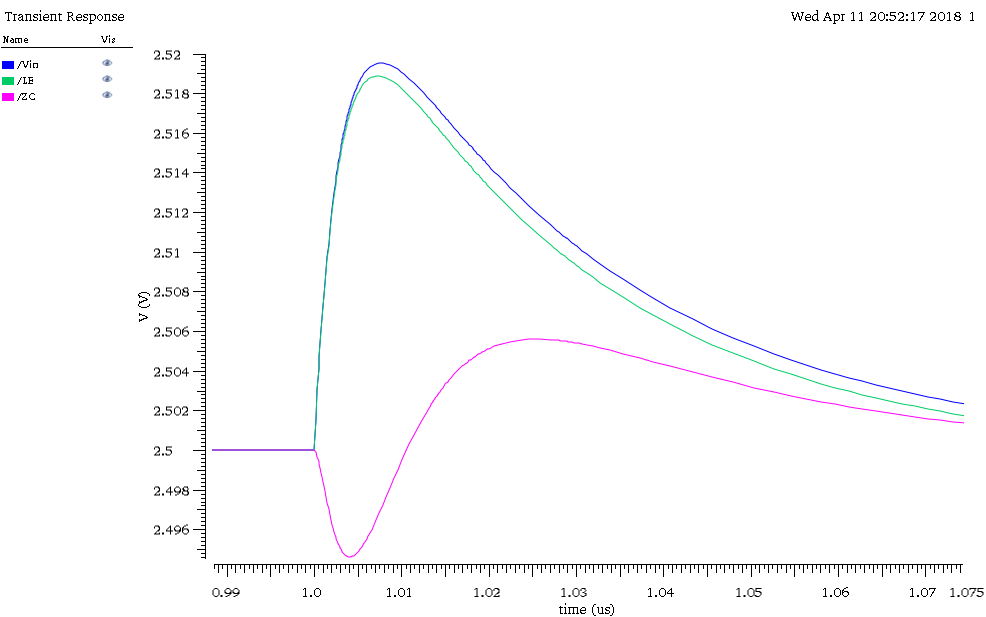
\includegraphics[scale=.55,keepaspectratio=true]{data/nowlin_3n_atten.png}
\caption{Nowlin attenuation of 3 nsec input pulse}
\label{fig:atten3}
\end{figure}
\newpage
\begin{figure}[htbp!]
\centering
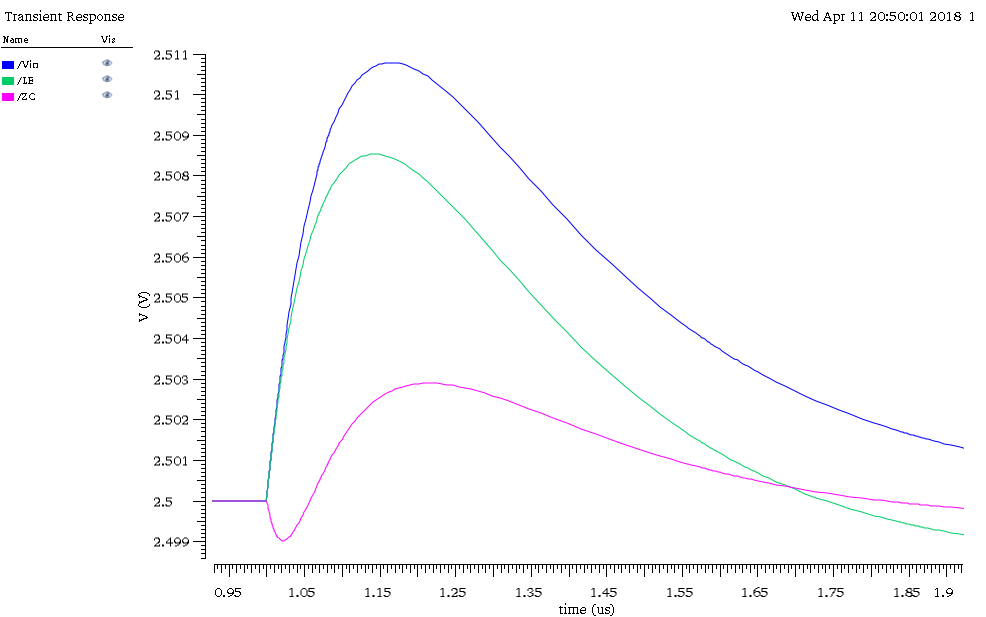
\includegraphics[scale=.55,keepaspectratio=true]{data/nowlin_100n_atten.png}
\caption{Nowlin attenuation of 100 nsec input pulse}
\label{fig:atten100}
\end{figure}
\section{Differential Amplifier}
%required spec
%diffamp GBW, output swing, frequency response
\par The performance of the differential amplifier is critical for the operation of both the LED and ZCD circuits. The GBW needs to be at least 175 MHz to avoid attenuation of the input differential signal and allow for a 50 MHz bandwidth after cascading three diffamps together in the ZCD \cite{CFD}. The diffamp also needs an output voltage swing between 0.75 and 2.5 V. 
\subsection{Frequency Response}
\par Figure~\ref{fig:freq} shows the frequency response of the diffamp under a typical design corner. The GBW is $\approx$ 620 MHz, with a phase margin of 84 degrees when loaded with another diffamp. The diffamp has a low frequency open loop gain greater than 80 dB at all corners (worst case speed, worst case power). 
\begin{figure}[htbp!]
\centering
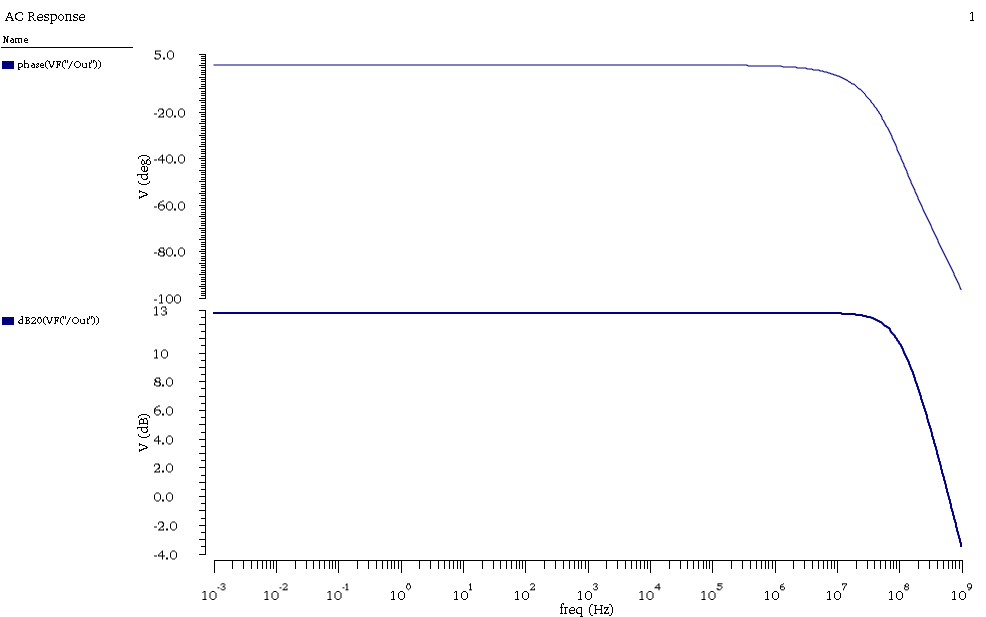
\includegraphics[scale=.55,keepaspectratio=true]{images/diffamp_mag_phase.png}
\caption{Frequency response of diffamp.}
\label{fig:freq}
\end{figure}
\subsection{Noise}
\par The thermal noise at the output of the differential amplifier is $\approx$ 70 $\mu V$ in worst case. The $\frac{1}{f}$ noise between 1 mHz and 1 GHz is 130 $\mu V$. The total integrated noise can then be calculated by Eqn~\ref{eq:noise} \cite{ALLEN-HOLBERG}.
\begin{align}
\sigma _{ v} = \sqrt{\sigma _{f^{-1}}^{2} + \sigma _{t}^{2}} \approx 150 \mu V
\label{eq:noise}
\end{align}
\subsection{Output swing}
\par The output voltage swing of the differential amplifier is 0.4 V to 3.1 V for typical design corners. Under worst case speed and worst case power the range drops to 0.5 to 2.8 V which still exceeds the design specification. 
\section{Comparator}
\par The comparator design needs a fast propagation delay and rise time for inputs between 20 mV and 2 V. Originally a comparator design using a large positive feedback stage was used under ideal circumstances and showed promising results. The design, shown in Figure~\ref{fig:feedback}, uses cross coupled NFETS to create a high gain stage to improve comparator speed and sensitivity \cite{BAKER}. However once simulations were ran including small systematic DC offsets the comparator no longer functioned due to the large ($\approx 120,000$) gain causing the output to stick to one of the supply rails. 
\par The comparator was redesigned without the positive feedback stage and could properly handle DC offset voltages of $\pm$ 4 mV without latching into a single output state. This comparator design has rise times of 200 psec and a propagation delay of $\approx$ 3 nsec.
\begin{figure}[htbp!]
\centering
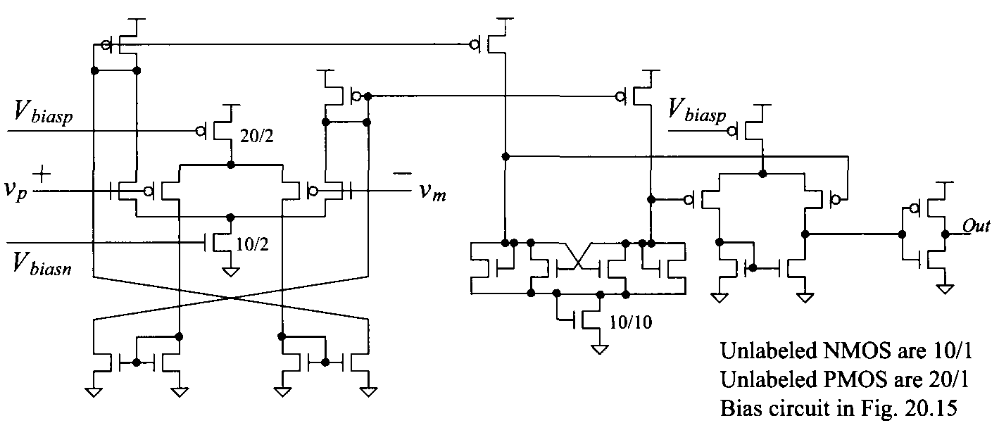
\includegraphics[scale=.55,keepaspectratio=true]{images/old_comp.png}
\caption{Comparator with positive feedback stage.}
\label{fig:feedback}
\end{figure}
\section{Output Walk \& Jitter}
\par The most important design constraint of the CFD16C is that the output timing pulse must have very low walk time and jitter. The walk time refers to the difference in output firing times as input amplitude changes. Jitter refers to variation in output firing times when amplitude remains constant \cite{CFD}. These design constraints influenced the design of most other circuits described thus far.
\subsection{Time Walk}
\par For a good time walk the ZCD needed to be optimized. The original design used five differential amplifier stages before the output comparator. While this worked well for low amplitude pulses, fast (ie. 3 nsec) large amplitude pulses suffered large propagation delays. Figure~\ref{fig:diffampdelay} shows the propagation delay results when using between 1 and 4 diffamp stages. As can be seen, more diffamp stages improves response at lower amplitudes but becomes increasingly nonlinear at higher amplitudes. 
\par Using two diffamp stages offers the best linearity and walk times however the reduced gain hurt the performance at worst case design corners. The final ZCD design uses 3 stages as a best compromise between fast propagation for small amplitudes and linearity at higher amplitudes.
\begin{figure}[htbp!]
\centering
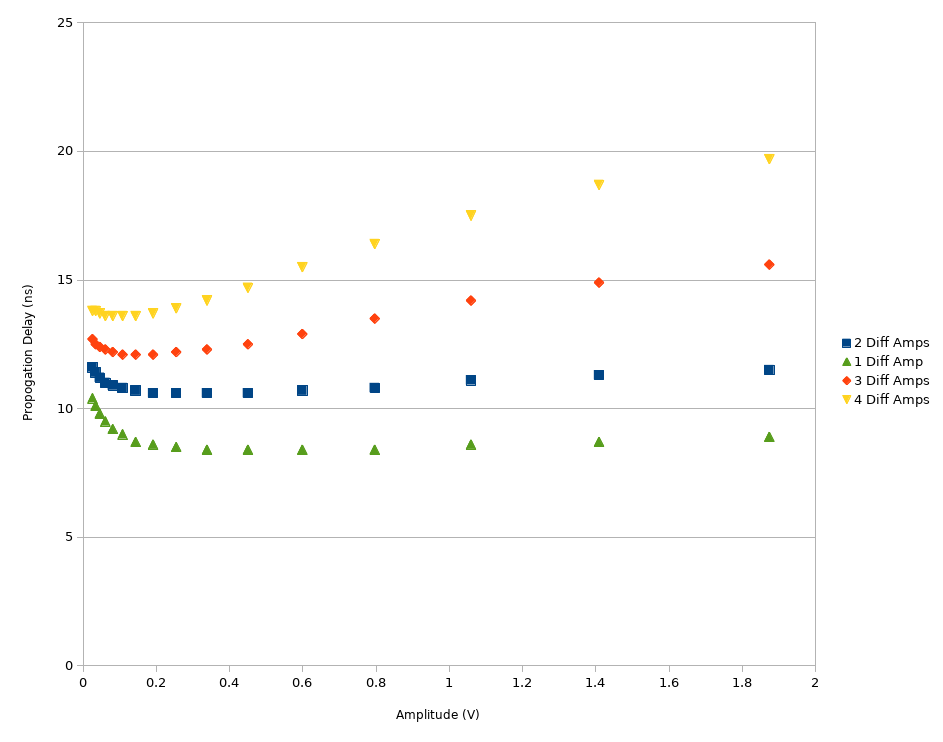
\includegraphics[scale=.55,keepaspectratio=true]{data/propogation.png}
\caption{Relationship between propagation delay and number of diffamp stages.}
\label{fig:diffampdelay}
\end{figure}
\par With three diffamp stages the walk times are not perfect at higher amplitudes. The design target of less than 1 nsec is only met for amplitudes under 600 mV. However since the 1 nsec walk times are most critical at lower amplitudes this was determined to be an acceptable compromise. Table~\ref{tab:walk3n} shows the firing times for 3 nsec pules while Table~\ref{tab:walk100n} shows walk times for 100 nsec pulses. The final walk times for input pulses between 20 mV and 600 mV was 800 psec (3.5 nsec at 2 V) for 3 nsec rise times. For 100 nsec rise times the 20-600 mV range walk time was 3 nsec (3.5 nsec at 2 V).
\par While these walk times are not ideal, they are acceptable for the intended applications of the CFD16C. The walk times for fast rise times is more critical than for slow rise times and the performance is optimized more for the smaller amplitude input pulses. 
\begin{table}[h]
\parbox{.45\linewidth}{
\centering
	\begin{tabular}{|l|p{4cm}|}
		\hline
		Amplitude (V) & Propagation delay (nsec)\\\hline
		0.026 & 12.7\\\hline
		0.035 & 12.5\\\hline
		0.046 & 12.4\\\hline
		0.061 & 12.3\\\hline
		0.081 & 12.2\\\hline
		0.11 & 12.1\\\hline
		0.14 & 12.1\\\hline
		0.19 & 12.1\\\hline
		0.25 & 12.2\\\hline
		0.34 & 12.3\\\hline
		0.45 & 12.5\\\hline
		0.6 & 12.9\\\hline
		0.8 & 13.5\\\hline
		1 & 14.2\\\hline
		1.4 & 14.9\\\hline
		1.9 & 15.6\\\hline
	\end{tabular}
    \caption{3 nsec walk times}
 	\label{tab:walk3n}
 	}
 	\hfill
\parbox{.45\linewidth}{
	\begin{tabular}{|l|p{4cm}|}
		\hline
		Amplitude (V) & Propagation delay (nsec)\\\hline
		0.026 & 17\\\hline
		0.035 & 16.6\\\hline
		0.046 & 16.2\\\hline
		0.061 & 15.8\\\hline
		0.081 & 15.6\\\hline
		0.11 & 15.2\\\hline
		0.14 & 14.9\\\hline
		0.19 & 14.7\\\hline
		0.25 & 14.5\\\hline
		0.34 & 14.3\\\hline
		0.45 & 14.1\\\hline
		0.6 & 14\\\hline
		0.8 & 13.9\\\hline
		1 & 13.7\\\hline
		1.4 & 13.6\\\hline
		1.9 & 15.5\\\hline
	\end{tabular}
    \caption{100 nsec walk times.}
 	\label{tab:walk100n}
    }
\end{table}
\subsection{DC Offsets}
\par The walk times in the previous section were obtained using ideal simulations without DC systematic DC offset voltages factored in. Walk times were also obtained after introducing small DC offset voltages at the input of the first diffamp stage in the ZCD. Figure ~\ref{fig:dcoff} shows the walk plot for a 20 mV pulse with different DC offset voltages applied. It can easily be seen the DC offset voltages do not affect the walk times in any appreciable way.
\subsection{Jitter}

\chapter{SUMMARY, CONCLUSIONS, AND FUTURE WORK}

\section{Summary}
\par The CFD16C will implement configurable discriminator channels to support up to 16 detectors. The IC is a companion chip for the PSD8C (also designed in the SIUE VLSI research lab), designed to mark the arrival times of an input pulse to start time-to-voltage converters on the PSD8C. Each channel will provide an accurate timing pulse that is independent of pulse amplitude and rise time, with walk times of less than 1 nsec and low jitter (sub 300 psec).
\par The sixteen identical channels are composed of five stages. 
\begin{enumerate}
\item
Nowlin input stage to create differential output for zero crossing discriminator.
\item
Leading edge discriminator stage to qualify the output of the zero crossing discriminator and guarantee output only from an input pulse.
\item
Zero crossing discriminator stage to create output pulse independent of input pulse amplitude.
\item
Oneshot stage to create the output timing pulse.
\item
Output stage to create all of the channel outputs.
\end{enumerate}

\par Each channel will be configurable independently of the others due to an addressing and mode scheme allowing for channels and individual registers to be addressed. Global configuration for Nowlin circuit delay, and test point channel select are also available in a common channel. The design presented in this thesis was done in the AMIS 0.5-micron process.

\section{Conclusions}
\par A time walk of less than 1 ns regardless of pulse amplitude and rise time is clearly achievable in 0.5-micron CMOS. Simulated data shows the CFD16C would work as intended if work were to continue in this design process.

\section{Future Work}
\par  The CFD16C design presented here will not be fabricated. The designs will instead be translated over to the newer 0.35 micron AMS process. As of this writing work has already started on translating these designs over to this newer process. 
\par The CFD16C its self is not a complete design. There are many circuits missing form this thesis as they were not finished before switching over to the new AMS design process. The ZCD will contain a DC offset cancellation loop to help remove systematic DC offset voltages in the diffamp stages. The 6-bit DAC for the LED has also been redesigned using an R2R ladder topology in the new AMS process. Work will continue on the CFD16C to be fabricated in the AMS process. The CFD16C will likely be ready for fabrication by mid 2018. Once fabricated the CFD16C will be thoroughly tested to ensure it works as simulated. Should there be discrepancies in the real world data and simulated data, new simulations will be run to identify the cause. 

\references %single spacing / arabic numeral paginations, adds "REFERENCES" to table of contents

%%%% for bibtex

%If you want to use bibtex  use the following lines, where your .bib file is called 'yourbib.bib'

\bibliographystyle{apalike}
\bibliography{./borabut_thesis.bib}

% If you have only a single appendix, do it this way.

\multipleappendices
\lstset{
         language=C,
         basicstyle=\scriptsize\ttfamily,
         emptylines=0, 
         lineskip=1pt,
         %numbers=left,            
         numberstyle=\tiny,         
         stepnumber=2,              
         numbersep=5pt,             
         tabsize=3,                
         extendedchars=true,       
         breaklines=true,            
         commentstyle=\color{blue},
         keywordstyle=\color{red},
            frame=b,         
 %        keywordstyle=[1]\textbf,    
 %        keywordstyle=[2]\textbf,    
 %        keywordstyle=[3]\textbf,  
 %        keywordstyle=[4]\textbf,   \
         stringstyle=\scriptsize\color{green}\ttfamily, 
         showspaces=false,         
         showtabs=false,            
%         xleftmargin=17pt,
%         framexleftmargin=17pt,
%         framexrightmargin=5pt,
%         framexbottommargin=4pt,
         %backgroundcolor=\color{lightgray},
         showstringspaces=false           
 }

\chapter{Verilog-A Code}

\end{document}